\chapter{Разработка метода тактильного очувствления}\label{ch:ch4}

Четвертая глава раскрывает детали создания алгоритма построения карты с помощью тактильного очувствления, определения типа поверхности.

Для реализации блока <<построение модели поверхности>>, необходимы входные данные, которые были  описаны в главе \nameref{ch:ch3}. Для определения геометрических свойств поверхности необходимо получить облако точек касаний опорных поверхностей. То есть мы должны знать трансформацию систем координат от глобальной (к примеру начало движения робота), до конкретного сенсора на ноге. Это возможно сделать, решив задачу кинематики и локализации робота.

\begin{figure}[H]
    \centering
     \begin{tikzpicture}
        % Include the image in a node
        \node [above right, inner sep=0] (image) at (0,0) 
        {\centering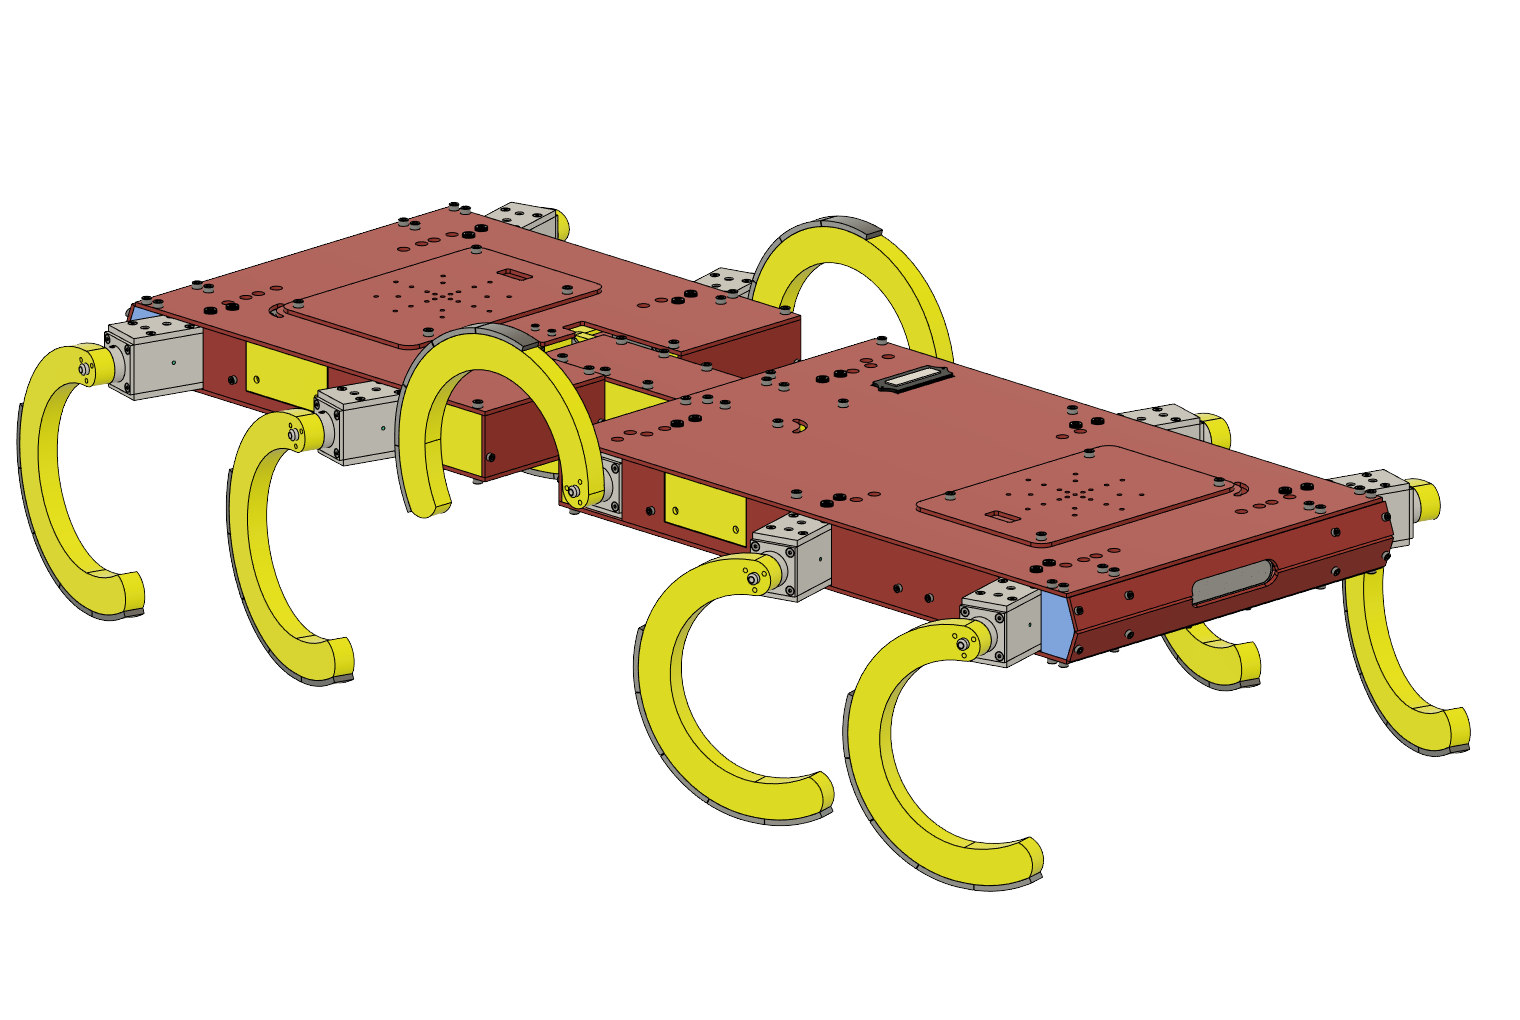
\includegraphics[height=10cm,width=1\textwidth,keepaspectratio]{StriRus_10_legs_15_angle_v4.png}};          
        % Create scope with normalized axes
        \begin{scope}[
            x={($ 0.1*(image.south east)$)},
            y={($ 0.1*(image.north west)$)}]
            % Grid and axes' labels
            % \draw[lightgray,step=1] (image.south west) grid (image.north east);
            % \foreach \x in {0,1,...,10} { \node [below] at (\x,0) {\x}; }
            % \foreach \y in {0,1,...,10} { \node [left] at (0,\y) {\y};}
 
            % Labels

            \coordinate (Xc) at (0.4415/2,-0.2347/2);
            \coordinate (Yc) at (-0.4512/2,-0.2156/2);
            \coordinate (Zc) at (0,0.5/2);
            % Labels
            \tikzstyle{origin} = [rounded corners=2pt, black, fill=gray!40, fill opacity=0.75, text opacity=1, scale=0.8,inner sep=1pt]
            \tikzstyle{transform_text} = [rounded corners=2pt, black, fill=white!85!gray, fill opacity=0.75, text opacity=1, scale=0.8,inner sep=1pt]
            \tikzstyle{transform_arrow} = [thick, green]
    
            % \coordinate (o_g) at (1,9);
            \node[circle,fill=green,scale=0.25] (o_g) at (1,9){};
            \draw[-stealth, very thick,blue] (o_g) -- ++(Xc);
            \draw[-stealth, very thick,green!70!black] (o_g) -- ++(Yc);
            \draw[-stealth, very thick,red] (o_g) -- ++(Zc);
            \node[origin,above right=3pt] at (o_g){\tiny $\mathbf{O_{glob}}$};
    
            % \coordinate (o_b) at (2.9,7.05);
            \node[circle,fill=green,scale=0.25] (o_b) at (2.9,7.05){};
            \draw[-stealth, very thick,blue] (o_b) -- ++(Xc);
            \draw[-stealth, very thick,green!70!black] (o_b) -- ++(Yc);
            \draw[-stealth, very thick,red] (o_b) -- ++(Zc);
            \node[origin,above right=2pt] at (o_b){\tiny $\mathbf{O_{base}}$};
    
            % \coordinate (o_1) at (2.9,6.6);
            \node[circle,fill=green,scale=0.25] (o_1) at (2.9,6.6){};
            \draw[-stealth, very thick,blue] (o_1) -- ++(Xc);
            \draw[-stealth, very thick,green!70!black] (o_1) -- ++(Yc);
            \draw[-stealth, very thick,red] (o_1) -- ++(Zc);
            \node[origin,above right=2pt] at (o_1){\tiny $\mathbf{O_{1}}$};
    
            % \coordinate (o_2) at (4,6);
            \node[circle,fill=green,scale=0.25] (o_2) at (4,6){};
            \draw[-stealth, very thick,blue] (o_2) -- ++(Xc);
            \draw[-stealth, very thick,green!70!black] (o_2) -- ++(Yc)
            node[origin,below=2pt]{\tiny $\mathbf{\alpha_3}$};
            \draw[-stealth, very thick,red] (o_2) -- ++(Zc);
            \node[origin,above right=2pt] at (o_2){\tiny $\mathbf{O_{2}=O_{3}}$};
    
            % \coordinate (o_4) at (7.0,4.55);
            \node[circle,fill=green,scale=0.25] (o_4) at (7.0,4.55){};
            \draw[-stealth, very thick,blue] (o_4) -- ++(Xc);
            \draw[-stealth, very thick,green!70!black] (o_4) -- ++(Yc);
            \draw[-stealth, very thick,red] (o_4) -- ++(Zc);
            \node[origin,above right=2pt] at (o_4){\tiny $\mathbf{O_{4}}$};
    
            % \coordinate (o_5) at (6.7,4.45);
            \node[circle,fill=green,scale=0.25] (o_5) at (6.7,4.45){};
            \draw[-stealth, very thick,blue] (o_5) -- ++(Xc);
            \draw[-stealth, very thick,green!70!black] (o_5) -- ++(Yc);
            \draw[-stealth, very thick,red] (o_5) -- ++(Zc);
            \node[origin,above left=3pt] at (o_5){\tiny $\mathbf{O_{5}=O_{6}}$};
    
            \coordinate (Xcr) at (0.49/2,0.07/2);
            % \coordinate (Ycr) at (-0.38/2,-0.32/2);
            \coordinate (Ycr) at (-0.24/2,-0.43/2);
    
            \draw[-stealth, very thick,blue] (o_5) -- ++(Xcr);
            \draw[-stealth, very thick,green!70!black] (o_5) -- ++(Ycr);
    
    
            % \coordinate (o_7) at (6.36,3.68);
            \node[circle,fill=green,scale=0.25] (o_7) at (6.36,3.68){};
            \draw[-stealth, very thick, blue] (o_7) -- ++(Xcr);
            \draw[-stealth, very thick, green!70!black] (o_7) -- ++(Ycr)
            node[origin,above left=2pt]{\tiny $\mathbf{\alpha_8}$};
            \draw[-stealth, very thick, red] (o_7) -- ++(Zc);
            \node[origin,below right=3pt] at (o_7){\tiny $\mathbf{O_{7}=O_{8}}$};
    
            \node[circle, draw ,fill=green,scale=0.4] (s_1) at (6.6,1.3){1};
            \node[circle,draw, fill=green,scale=0.4] (s_3) at (5.85,1.7){3};
            \node[circle,draw, fill=green,scale=0.4] (s_5) at (5.55,2.9){5};
    
            \draw[-stealth, transform_arrow] (o_g) -- (o_b)
            node[midway,below left=2pt, transform_text]{\tiny $\mathbf{H_{base}^{glob}}$};
    
            \draw[-stealth, transform_arrow] (o_b) -- (o_1)
            node[midway,left=3pt, transform_text]{\tiny $\mathbf{H_{1}^{base}}$};
    
            \draw[-stealth, transform_arrow] (o_1) -- (o_2)
            node[midway,below=2pt, transform_text]{\tiny $\mathbf{H_{2}^{1}}$};
    
            \draw[-stealth, transform_arrow] (o_2) -- (o_4)
            node[midway,below=2pt, transform_text]{\tiny $\mathbf{H_{4}^{3}}$};
    
            \draw[-stealth, transform_arrow] (o_4) -- (o_5)
            node[midway,below right=2pt, transform_text]{\tiny $\mathbf{H_{5}^{4}}$};
    
            \draw[-stealth, transform_arrow] (o_5) -- (o_7)
            node[midway,left=3pt, transform_text]{\tiny $\mathbf{H_{7}^{6}}$};
    
            \draw[-stealth, transform_arrow] (o_7) -- (s_1);
            \draw[-stealth, transform_arrow] (o_7) -- (s_3);
            \draw[-stealth, transform_arrow] (o_7) -- (s_5);
        \end{scope}
    \end{tikzpicture}
    \caption{Кинематическая схема для определения точки касания опорной поверхности роботом}
    \label{fig:StriRus_10_legs_15_angle_v4.png}
\end{figure}

\begin{multline}
        H_{leg}^{glob} = H(x_{glob},y_{glob},z_{glob},\alpha_{glob},\beta_{glob},\gamma_{glob})T_z(l_1)\\ T_x(l_2)R_y(\alpha_3)T_x(l_4)T_y(l_5)R_z(-15^{\circ})T_y(l_7)R_y(\alpha_8)
\end{multline}
Где каждая матрица представлены в виде однородной матрицы преобразования $H = \begin{bmatrix}
        \underset{3 \times 3}{R} & \underset{3 \times 1}{T} \\
        \underset{1 \times 3}{0} & \underset{1 \times 1}{1}
    \end{bmatrix}$, где $R_i$ --- матрица поворота, относительно одной из осей, $T_i$ --- вектор сдвига.
    
    Ниже представлены типы однородных матриц, которые могут быть встречены далее в высокоуровневых уравнениях. $H$ --- означает, что матрица содержит в себе одновременно и вращение и перемещение. $T_i$ --- подматрица поворота является единичной матрицей,а в векторе сдвига присутствует только один компонент под осью координат $i$, остальные значения равны $0$. При обозначении $R_i$ --- вектор сдвига равен нулю, а матрица поворота представляет поворот против часовой стрелки вокруг представленной оси вращения ${\displaystyle {\begin{alignedat}{1}R_{x}(\theta )&={\begin{bmatrix}1&0&0\\0&\cos \theta &-\sin \theta \\[3pt]0&\sin \theta &\cos \theta \\[3pt]\end{bmatrix}}\ R_{y}(\theta )&={\begin{bmatrix}\cos \theta &0&\sin \theta \\[3pt]0&1&0\\[3pt]-\sin \theta &0&\cos \theta \\\end{bmatrix}}\ R_{z}(\theta )&={\begin{bmatrix}\cos \theta &-\sin \theta &0\\[3pt]\sin \theta &\cos \theta &0\\[3pt]0&0&1\\\end{bmatrix}}\end{alignedat}}}$

    Таким образом, мы получаем матрицу, позволяющую получать координаты педипуляторов, относительно абсолютной системы координат. Матрица перехода учитывает подвижность самого педипулятора, а так же относительное изменение позиций сегментов.

\section{Картографирование с помощью ощупывания поверхности}
Определение геометрической модели поверхности позволяет оператору понимать примерные габариты пещеры, что позволит подготовить более специализированных роботов для решения исследовательских или поисковых задач.

Традиционно, карта для навигации представляется в виде облака точек. Тогда, без предложенного алгоритма, будут получено очень разреженное облако точек, где точки будут являться точками касания лапок робота с поверхностью.

Сделав предположение, что расстояние между ногами робота мало относительно целой пещеры, можно предположить, что поверхность, полученная как выпуклая оболочка, на основе точек контакта ног с поверхностью, является плоскостью.

Было выдвинуто ограничение, что робот движется по поверхности, у которой каждому набору координат $x,\ y$ соответствует одно и только одно значение координаты $z$. Что позволяет применять следующее уравнение $z=f(x,y)$. Обратная функция не действительна.

Для создания геометрической модели поверхности был разработан алгоритм, описанный далее. Вначале необходимо очистить оригинальное облако точек от шумов и усреднить близлежащие точки с помощью Voxel grid. Потом из него генерируется полигональная сетка с помощью 2D Триангуляции Делоне \pic{fig:delone_idea.png} (вогнутая оболочка \pic{fig:exp_concave_hull}). На ее основе получается необходимое плотное облако точек \pic{fig:sampled_pcd.png}.

\begin{figure}[H]
    \centering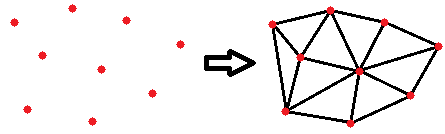
\includegraphics[height=5cm,width=1\textwidth,keepaspectratio]{delone_idea.png}
    \caption{2D Триангуляция Делоне (выпуклая оболочка)}
    \label{fig:delone_idea.png}
\end{figure}

Реализованный алгоритм проверялся, как в симуляции (Рис. \ref{fig:unsolvable_case}, \ref{fig:start_end_exp}), так и на реальном роботе \pic{fig:real_exp_map_creation}. Ссылка на видео представлена рядом \quad \qrcode[height=1.5cm]{https://youtu.be/2dxHHTG4psQ}.

Симуляция проводилась в CoppeliaSim, по причине того, симулятор отлично подходит для симуляции физики трения, что является ключевой частью корректной работы шагающих цикловых роботов. В симуляции использовался робот, состоящий из пяти пар ног и двух сегментов. Поверхность генерировалась случайным образом.


\begin{figure}[H]
    \begin{subfigure}[t]{0.49\textwidth}
        \centering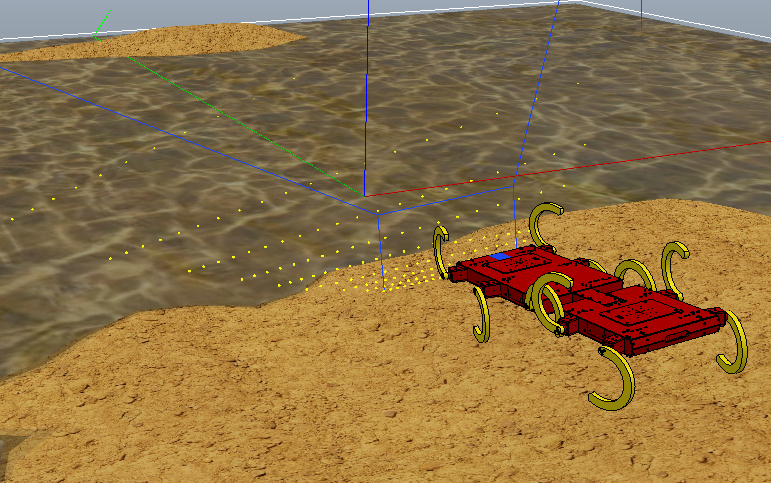
\includegraphics[height=5cm,width=1\textwidth,keepaspectratio]{terrain_w_water1.png}
        \caption{Начало движения}
    \end{subfigure}
    \begin{subfigure}[t]{0.49\textwidth}
        \centering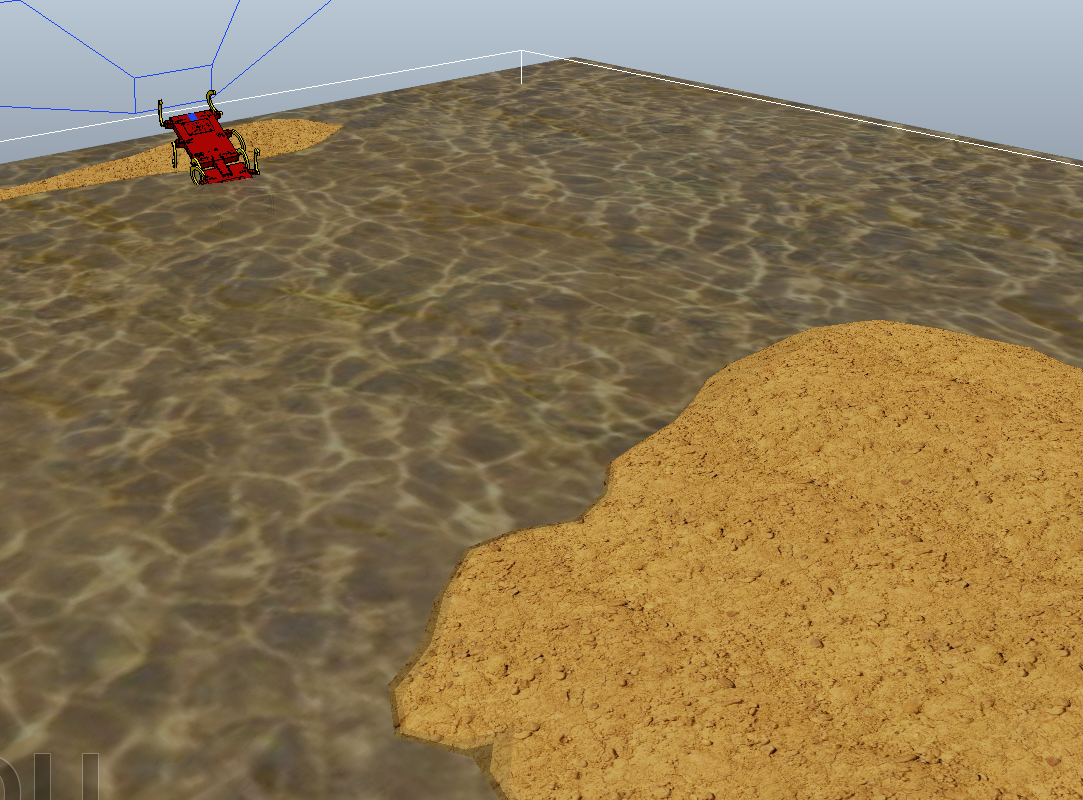
\includegraphics[height=5cm,width=1\textwidth,keepaspectratio]{terrain_w_water_end.png}
        \caption{Конец движения}
    \end{subfigure}
    \caption{Эксперимент в симуляторе}
    \label{fig:start_end_exp}
\end{figure}

Ниже представлены полученные результаты \pic{fig:result_meshes_blah}. Для оценки точности полученных данных использовались метрики C2C \eqref{eqn:hauff} и C2M \pic{fig:metrics}. Они основанны на метрике Хаусдорфа.


\begin{equation}
    \label{eqn:hauff}
    d_{H}(X,\;Y)=\sup _{m\in M}\left\{\,|\mathrm {dist} _{X}(m)-\mathrm {dist} _{Y}(m)|\,\right\}
\end{equation}
Где \nom{$X,\ Y$}{непустые подмножества метрического пространства $M$}; \nom{$\mathrm {dist} _{X}\colon M\to \mathbb {R}$}{обозначает функцию расстояния до множества $X$}.



\begin{figure}[H]
    \centering
        \begin{subfigure}[t]{0.4\textwidth}
            \centering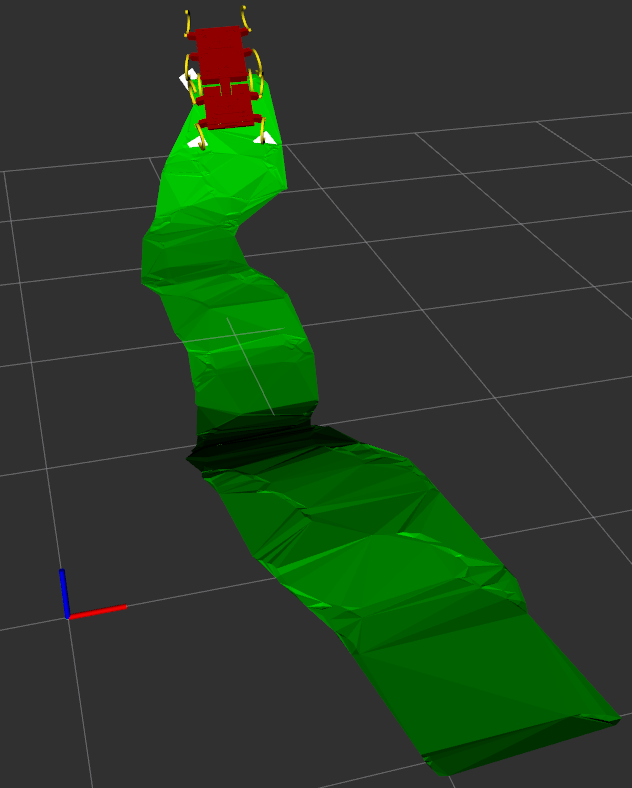
\includegraphics[height=8cm,width=1\textwidth,keepaspectratio]{mesh_rviz.png}
            \caption{Полигональная сетка, созданная 2D Триангуляцией Делоне (вогнутая оболочка)}
        \end{subfigure}
        \begin{subfigure}[t]{0.59\textwidth}
            \centering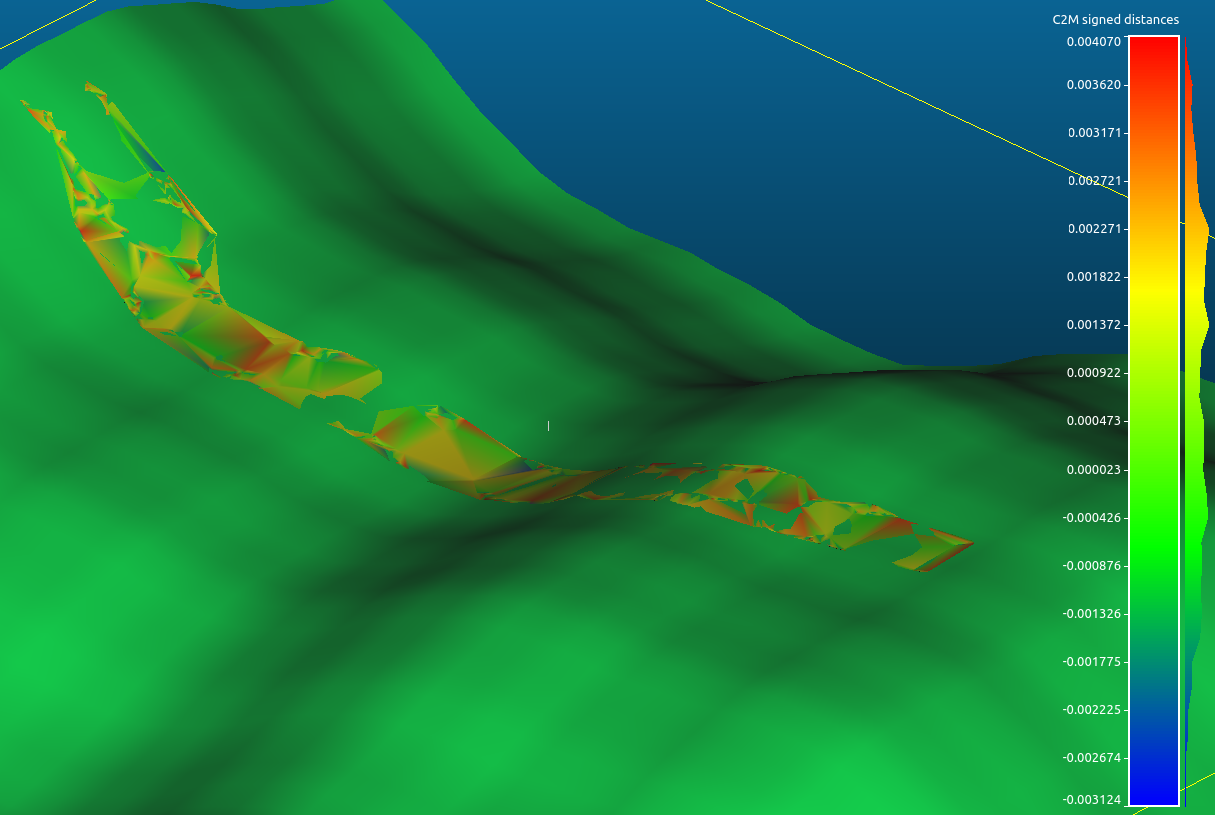
\includegraphics[height=8cm,width=1\textwidth,keepaspectratio]{mesh_comp.png}
            \caption{Наложенные полигональные сетки}
        \end{subfigure}

        \begin{subfigure}[t]{0.9\textwidth}
            \centering
            \begin{tikzpicture}
                % Include the image in a node
                \node [above right, inner sep=0] (image) at (0,0)
                {\centering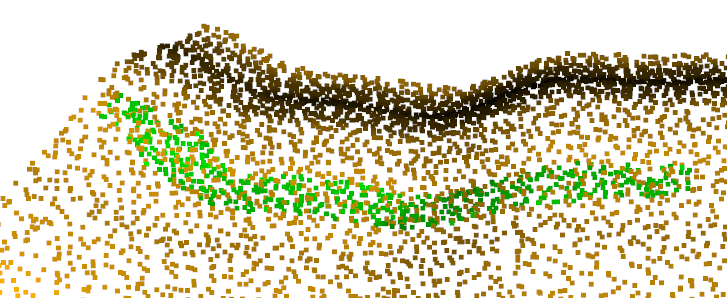
\includegraphics[height=8cm,width=1\textwidth,keepaspectratio]{sampled_pcd.png}};
                % Create scope with normalized axes
                \begin{scope}[
                        x={($ 0.1*(image.south east)$)},
                        y={($ 0.1*(image.north west)$)}]
                    \draw[stealth-, very thick,green] (3,8) -- (2,8.5);
                    \draw[stealth-, very thick,green] (1,5.5) -- (2,8.5)
                    node[rounded corners=3pt,above,black,fill=white]{\tiny Ground Truth Point Cloud};

                    \draw[stealth-, very thick,green] (5.5,3) -- (5.5,8.5)
                    node[rounded corners=3pt,above,black,fill=white]{\tiny Generated Point Cloud};
                \end{scope}
            \end{tikzpicture}
            \caption{Наложенные облака точек}
            \label{fig:sampled_pcd.png}
        \end{subfigure}
        \caption{Результат эксперимента}
        \label{fig:result_meshes_blah}
\end{figure}

\begin{figure}[H]
    \begin{subfigure}{0.9\textwidth}
        \centering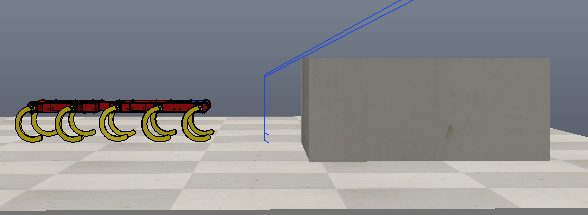
\includegraphics[height=8cm,width=1\textwidth,keepaspectratio]{postament_orig.png}
        \caption{Результат эксперимента по построению карты постамента, симулятор}
        \label{fig:postament_orig.png}
    \end{subfigure}
    \begin{subfigure}{0.9\textwidth}
        \centering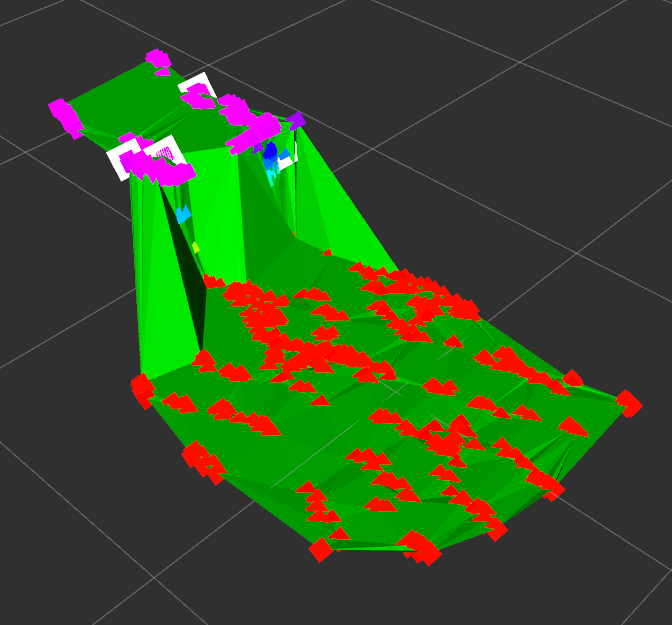
\includegraphics[height=8cm,width=1\textwidth,keepaspectratio]{postament_mesh.png}
        \caption{Результат эксперимента по построению карты постамента, Rviz, полигональная сетка}
        \label{fig:postament_mesh.png}
    \end{subfigure}

    \caption{Результат эксперимента по построению карты постамента}
    \label{fig:}
\end{figure}

На рисунке \ref{fig:exp_concave_hull} проиллюстрирована  важность модификации триангуляции Делоне. Как можно заметить \pic{fig:conv_convex.png} алгоритм построил карту местности неверно, расположив пройденную территорию там, где робот не перемещался и находится стена. При использовании вогнутой оболочки \pic{fig:conv_concave.png} данная проблема не наблюдается.

\begin{figure}[H]
    \begin{subfigure}[t]{0.3\textwidth}
        \centering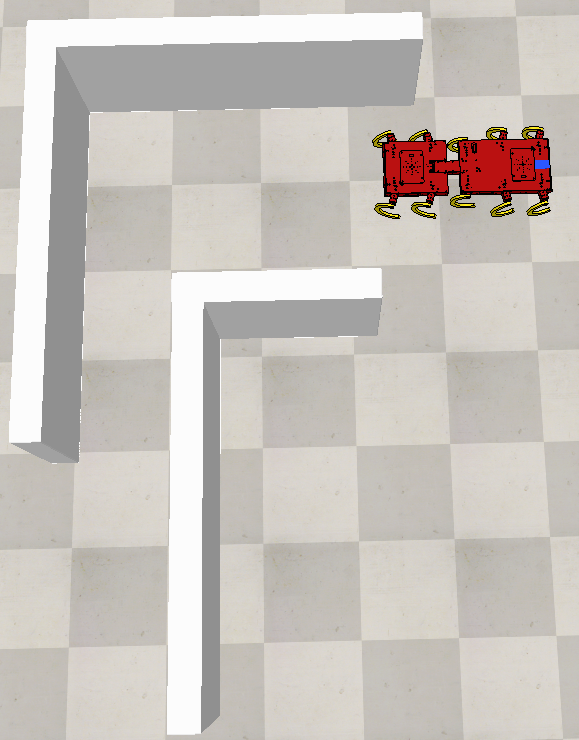
\includegraphics[height=8cm,width=1\textwidth,keepaspectratio]{convex_terr.png}
        \caption{Пример поля}
        \label{fig:convex_terr.png}
    \end{subfigure}
    \hfill
    \begin{subfigure}[t]{0.33\textwidth}
        \centering
        \begin{tikzpicture}
            % Include the image in a node
            \node [above right, inner sep=0] (image) at (0,0)
            {\centering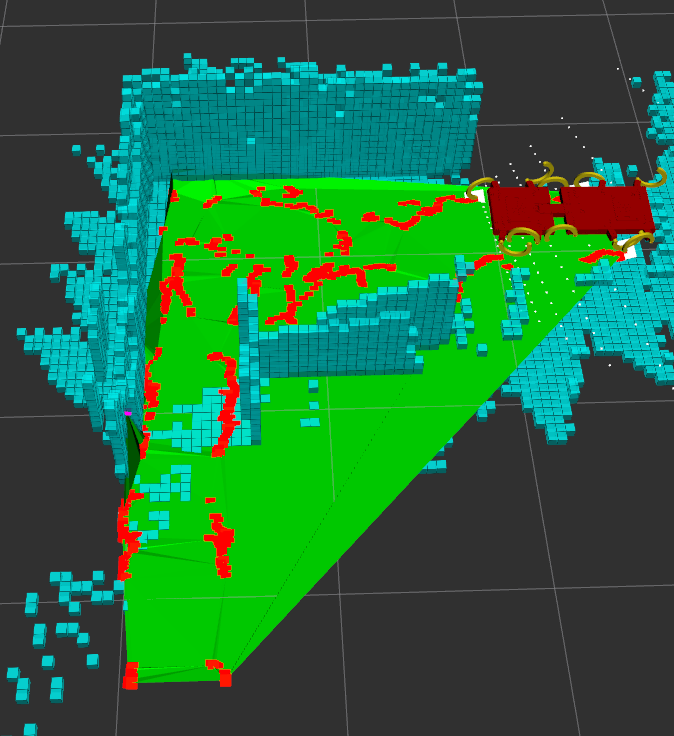
\includegraphics[height=8cm,width=1\textwidth,keepaspectratio]{conv_convex.png}};
            % Create scope with normalized axes
            \begin{scope}[
                    x={($ 0.1*(image.south east)$)},
                    y={($ 0.1*(image.north west)$)}]
                \draw[stealth-, very thick,green] (5.2,3.5) -- ++(1,-1)
                node[rounded corners=3pt,right,black,fill=white]{\tiny Generated mesh};

                \draw[stealth-, very thick,green] (5.5,5.5) -- (7.4,4)
                node[rounded corners=3pt,right,black,fill=white]{\tiny Lidar data};
                \draw[stealth-, very thick,green] (3.4,0.8) -- (5,1);
                \draw[stealth-, very thick,green] (3.4,2.6) -- (5,1)
                node[rounded corners=3pt,right,black,fill=white]{\tiny Cloud of contact points};
            \end{scope}
        \end{tikzpicture}
        \caption{Выпуклая оболочка}
        \label{fig:conv_convex.png}
    \end{subfigure}
    \hfill
    \begin{subfigure}[t]{0.30\textwidth}
        \centering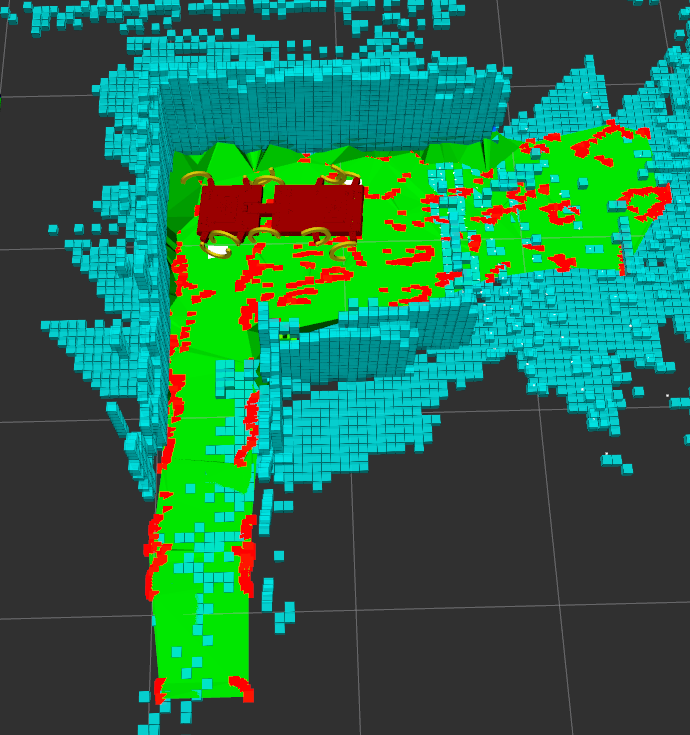
\includegraphics[height=8cm,width=1\textwidth,keepaspectratio]{conv_concave.png}
        \caption{Вогнутая оболочка}
        \label{fig:conv_concave.png}
    \end{subfigure}
    \caption{Объяснение необходимости модификации алгоритма Делоне}
    \label{fig:exp_concave_hull}
\end{figure}

\begin{figure}[H]
    \begin{subfigure}[t]{0.49\textwidth}
        \centering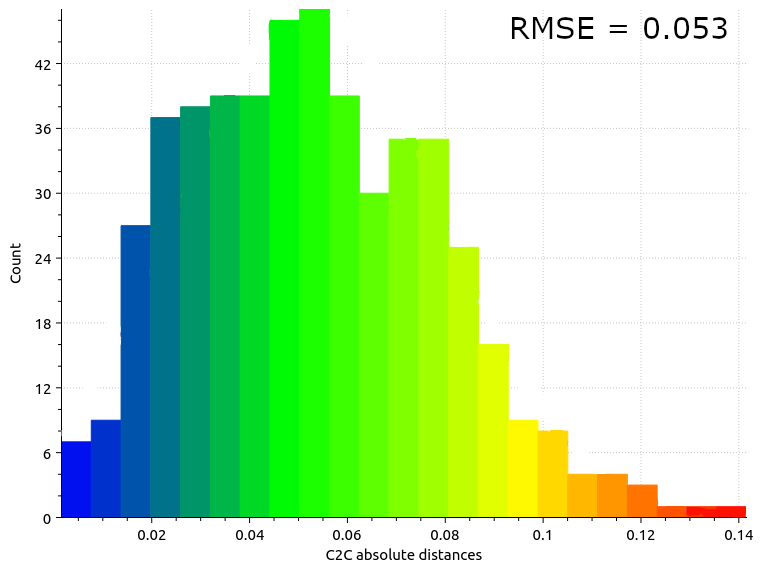
\includegraphics[height=8cm,width=1\textwidth,keepaspectratio]{pcd_hist.png}
        \caption{Метрика C2C: гистограмма ошибок (абсолютное расстояние от точки до ближайшей реферальной точки)}
        \label{fig:metric_c2c}
    \end{subfigure}
    \begin{subfigure}[t]{0.49\textwidth}
        \centering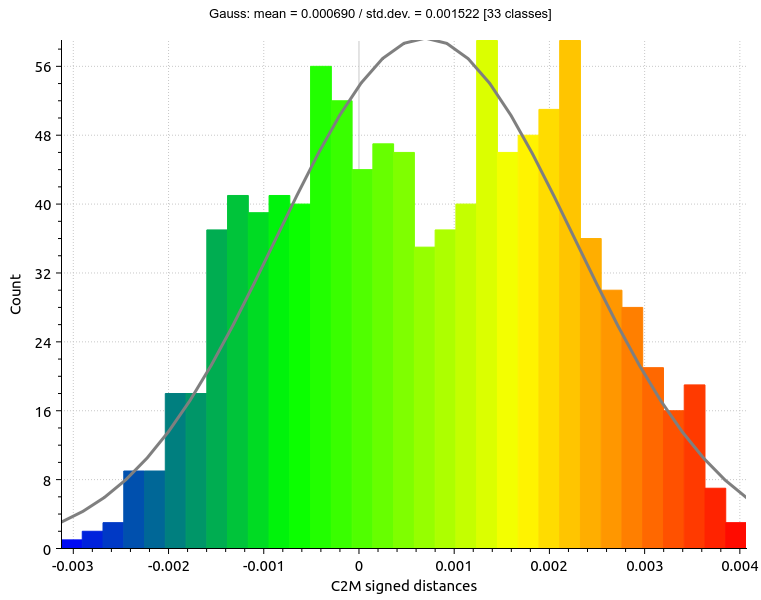
\includegraphics[height=8cm,width=1\textwidth,keepaspectratio]{mesh_hist.png}
        \caption{Метрика C2M: Гистограмма ошибок (относительное расстояние от точки до ближайшей реферальной точки)}
        \label{fig:metric_c2m}
    \end{subfigure}
    \caption{Метрики оценки точности полученной карты}
    \label{fig:metrics}
\end{figure}


\begin{figure}[H]
    \begin{subfigure}[t]{0.49\textwidth}
        \centering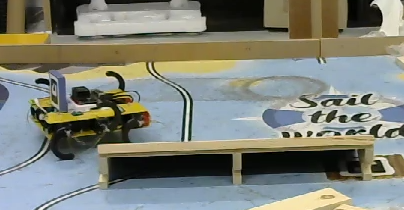
\includegraphics[height=8cm,width=1\textwidth,keepaspectratio]{real_robot_mesh_video_preview.png}
        \caption{Робот проходит препятствие}
        \label{fig:real_robot_mesh_video_preview.png}
    \end{subfigure}
    \begin{subfigure}[t]{0.49\textwidth}
        \centering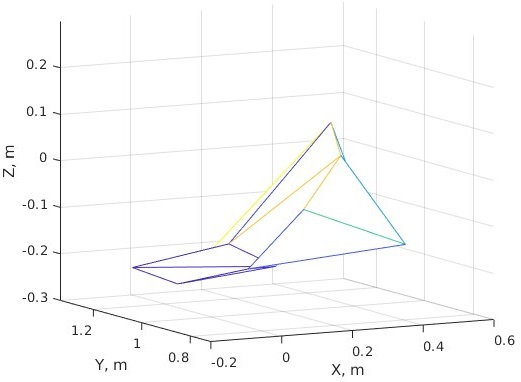
\includegraphics[height=8cm,width=1\textwidth,keepaspectratio]{real_mesh.jpg}
        \caption{Полученная полигональная сетка}
        \label{fig:real_mesh.jpg}
    \end{subfigure}
    \caption{Пример натурного эксперимента}
    \label{fig:real_exp_map_creation}
\end{figure}

Как итог, среднеквадратичная ошибка для C2C метрики была в среднем равна 5 см. А для C2M 1 см. В натурном эксперименте среднеквадратичная ошибка по метрике C2C --- 8 см.

\section{Определение типа поверхности}
Для определения физических свойств поверхности нужны данные с датчиков силы. Сильно улучшить показания помогут данные с гироскопов и акселерометров, а также момент с моторов. Определение физических свойств позволяет спелеологу узнать тип исследуемой поверхности, что важно для научных исследований и подбора оборудования. Также такое знание позволяет реализовать адаптивное управление роботом, что сильно увеличивает его активную проходимость по маршруту.

Задачу определения типа поверхности можно определить следующим образом. Робот идет по поверхности, и собирает данные с датчиков силы, с момента на моторе и IMU. На основе предварительного обучения, данные обрабатываются и кластеризуются, на основе предварительно определенной базе знаний территорий.

Задачу обучения удобнее всего проводить в лабораторных условиях. Экспериментальная установка соответствует следующим требованиям: возможность установить новые поверхность и сменять их быстро. Это нужно для легкого создания базы знаний поверхностей. Бесконечное движение, для скорости обучения. Узел с ногой должен быть взят с робота, чтобы не пришлось решать похожую задачу на роботе.

Все это было достигнуто благодаря разборному экспериментальному столу и двухстепенному механизму, который ходит по окружности \pic{fig:s_shape_leg/s_leg_setup.JPG}. Для бесконечного движения по кругу при малых скоростях был применен следующий инженерный приём. Были соединены две ноги робота в одну. На рисунке ниже \pic{fig:s_shape_leg/leg_design.png} показаны как установлены сенсоры на получившейся ноге.

\begin{figure}[H]
    \begin{subfigure}[t]{0.49\textwidth}
        \centering
        \begin{tikzpicture}
            % Include the image in a node
            \node [above right, inner sep=0] (image) at (0,0)
            {\centering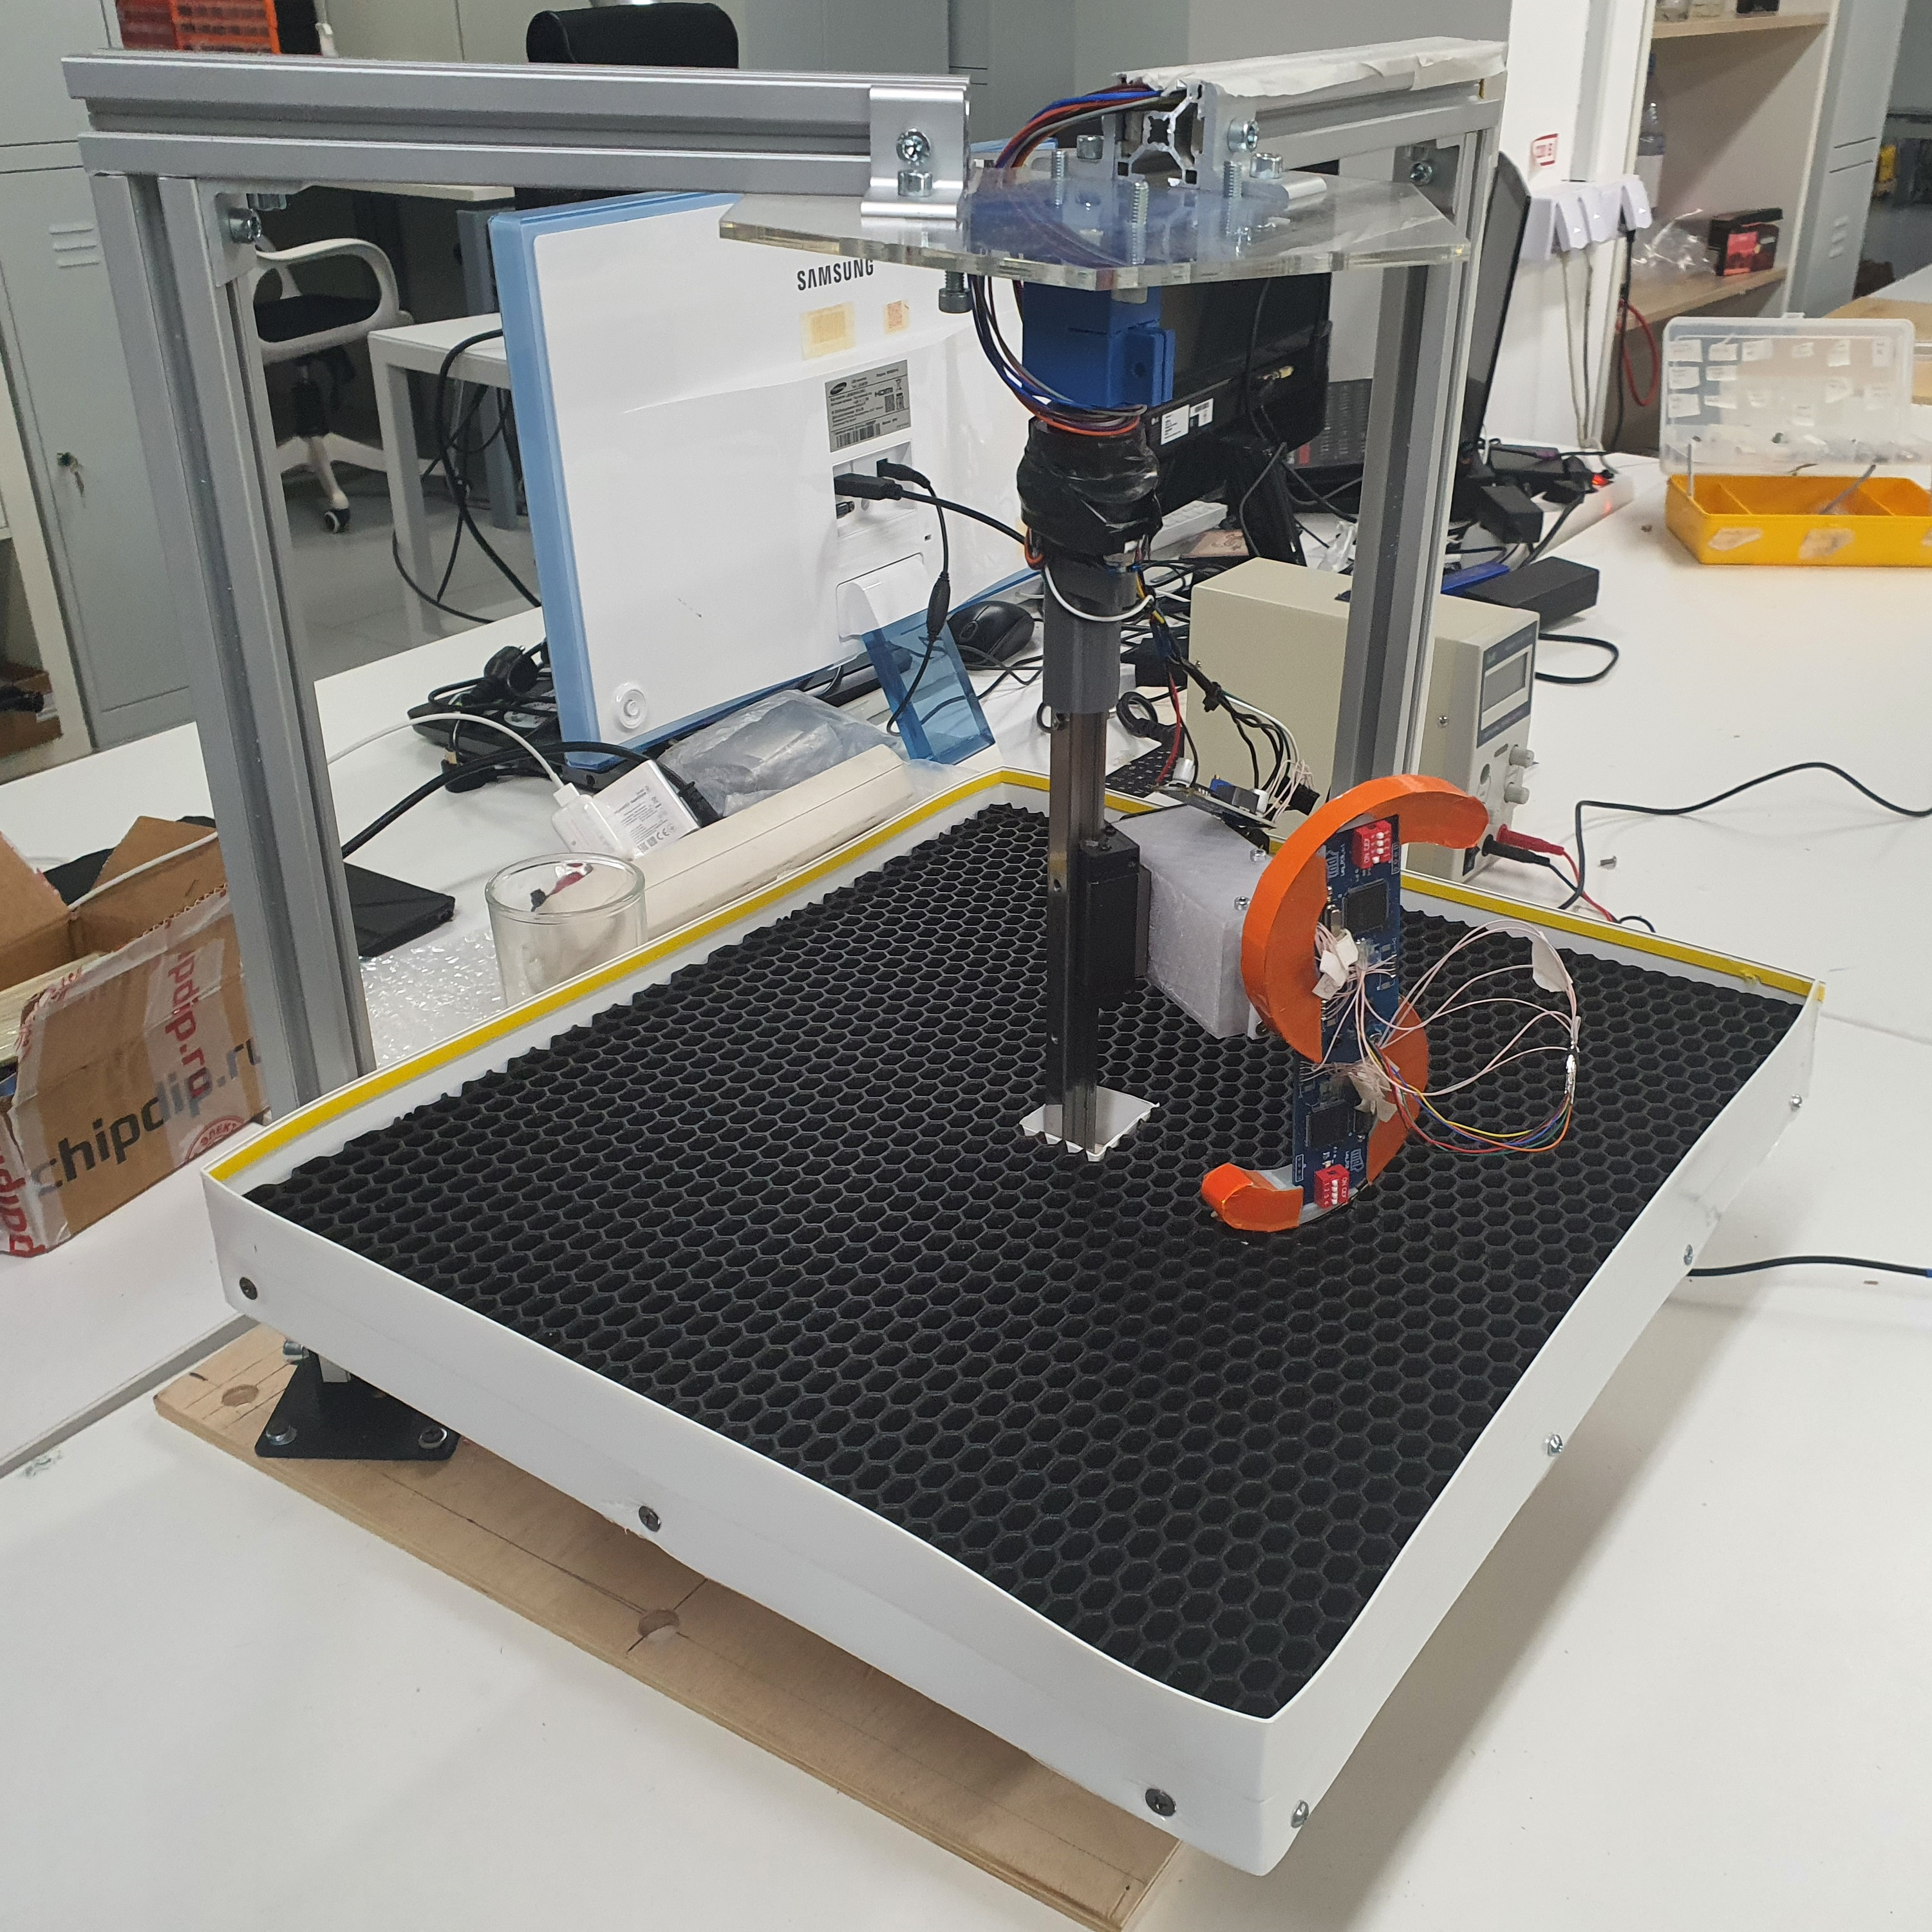
\includegraphics[height=8cm,width=1\textwidth,keepaspectratio]{s_shape_leg/s_leg_setup.JPG}};
            % Create scope with normalized axes
            \begin{scope}[
                    x={($ 0.1*(image.south east)$)},
                    y={($ 0.1*(image.north west)$)}]
                \draw[stealth-, very thick,green] (3.5,2.5) -- (3,1.5)
                node[rounded corners=3pt,below,black,fill=white]{\tiny Table for surfaces};

                \draw[stealth-, very thick,green] (7.1,5.4) -- (7.4,7)
                node[rounded corners=3pt,above right,black,fill=white]{\tiny Self-made PCB};

                \draw[very thick,green] (6,6.1) rectangle (8.5,3.5)
                node[above left,black,fill=green]{\tiny S leg};
            \end{scope}
        \end{tikzpicture}
        \caption{Общий вид экспериментальной установки}
        \label{fig:s_shape_leg/s_leg_setup.JPG}
    \end{subfigure}
    \begin{subfigure}[t]{0.49\textwidth}
        \centering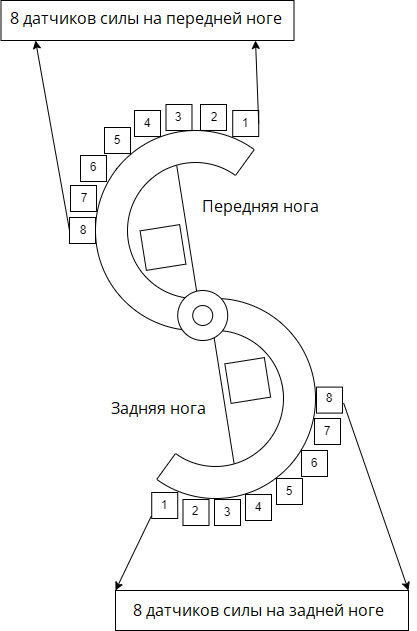
\includegraphics[height=8cm,width=1\textwidth,keepaspectratio]{s_shape_leg/leg_design.png}
        \caption{Пояснение по расположению сенсоров на ноге робота}
        \label{fig:s_shape_leg/leg_design.png}
    \end{subfigure}
    \caption{Экспериментальная установка для определения типа поверхности}
\end{figure}



Были взяты 3 сильно разных поверхности и изучены необработанные данные. Резина \pic{fig:s_shape_leg/s_leg_setup.JPG}  \quad \qrcode[height=1.5cm]{https://gifyu.com/image/SxatY} \quad, камень \pic{fig:s_shape_leg/view.jpg} \quad \qrcode[height=1.5cm]{https://gifyu.com/image/Sxatt}, земля \pic{fig:s_shape_leg/mould.jpg}.

\begin{figure}[H]
    \begin{subfigure}[t]{0.24\textwidth}
        \centering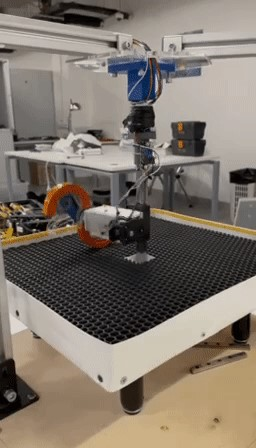
\includegraphics[height=9cm,width=1\textwidth,keepaspectratio]{s_shape_leg/flat.jpg}
        \caption{Резина}
        \label{fig:s_shape_leg/flat.jpg}
    \end{subfigure}
    \hfill
    \begin{subfigure}[t]{0.32\textwidth}
        \centering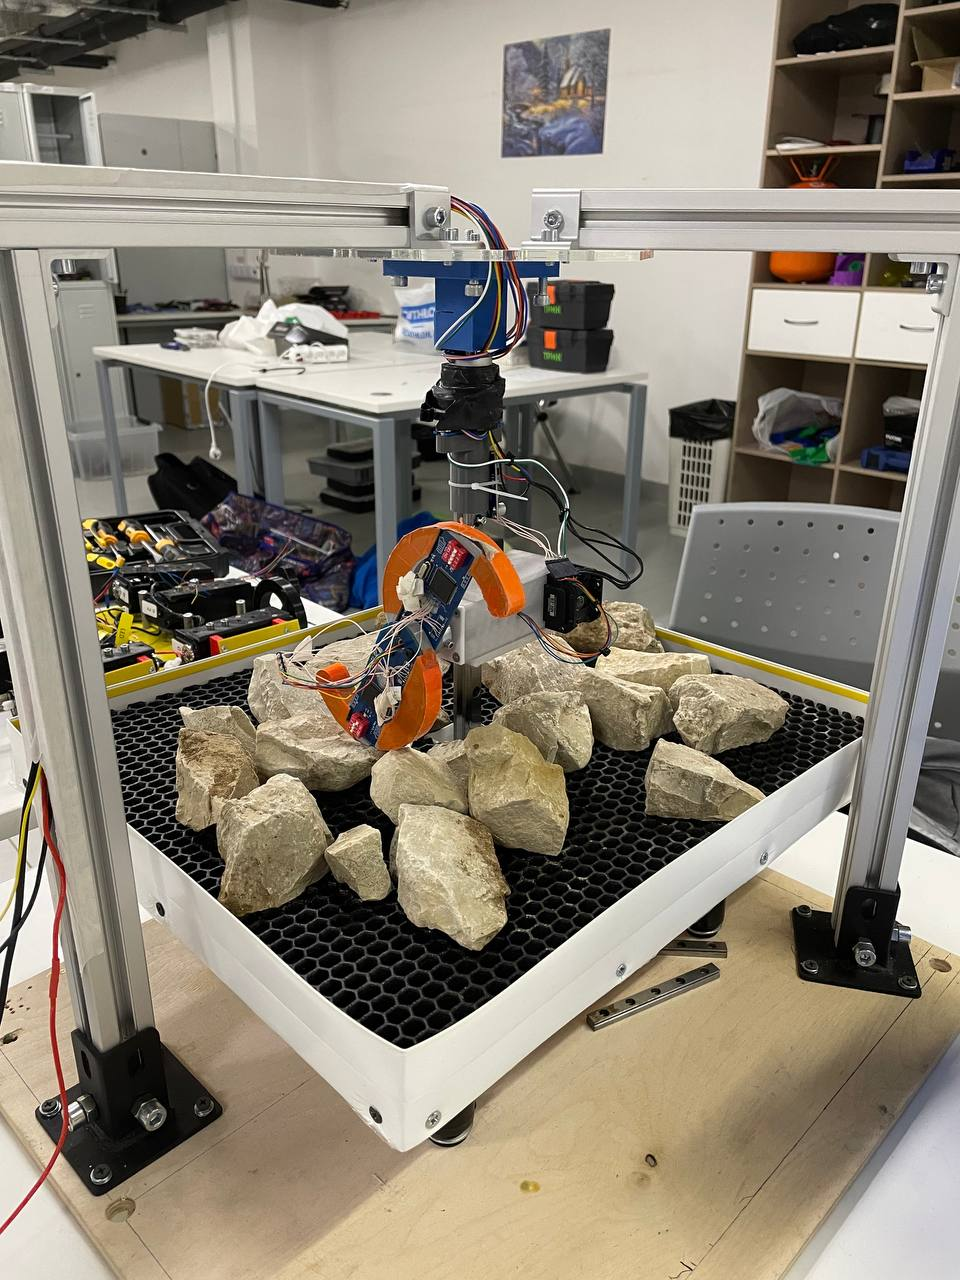
\includegraphics[height=9cm,width=1\textwidth,keepaspectratio]{s_shape_leg/view.jpg}
        \caption{Каменистая поверхность}
        \label{fig:s_shape_leg/view.jpg}
    \end{subfigure}
    \begin{subfigure}[t]{0.42\textwidth}
        \centering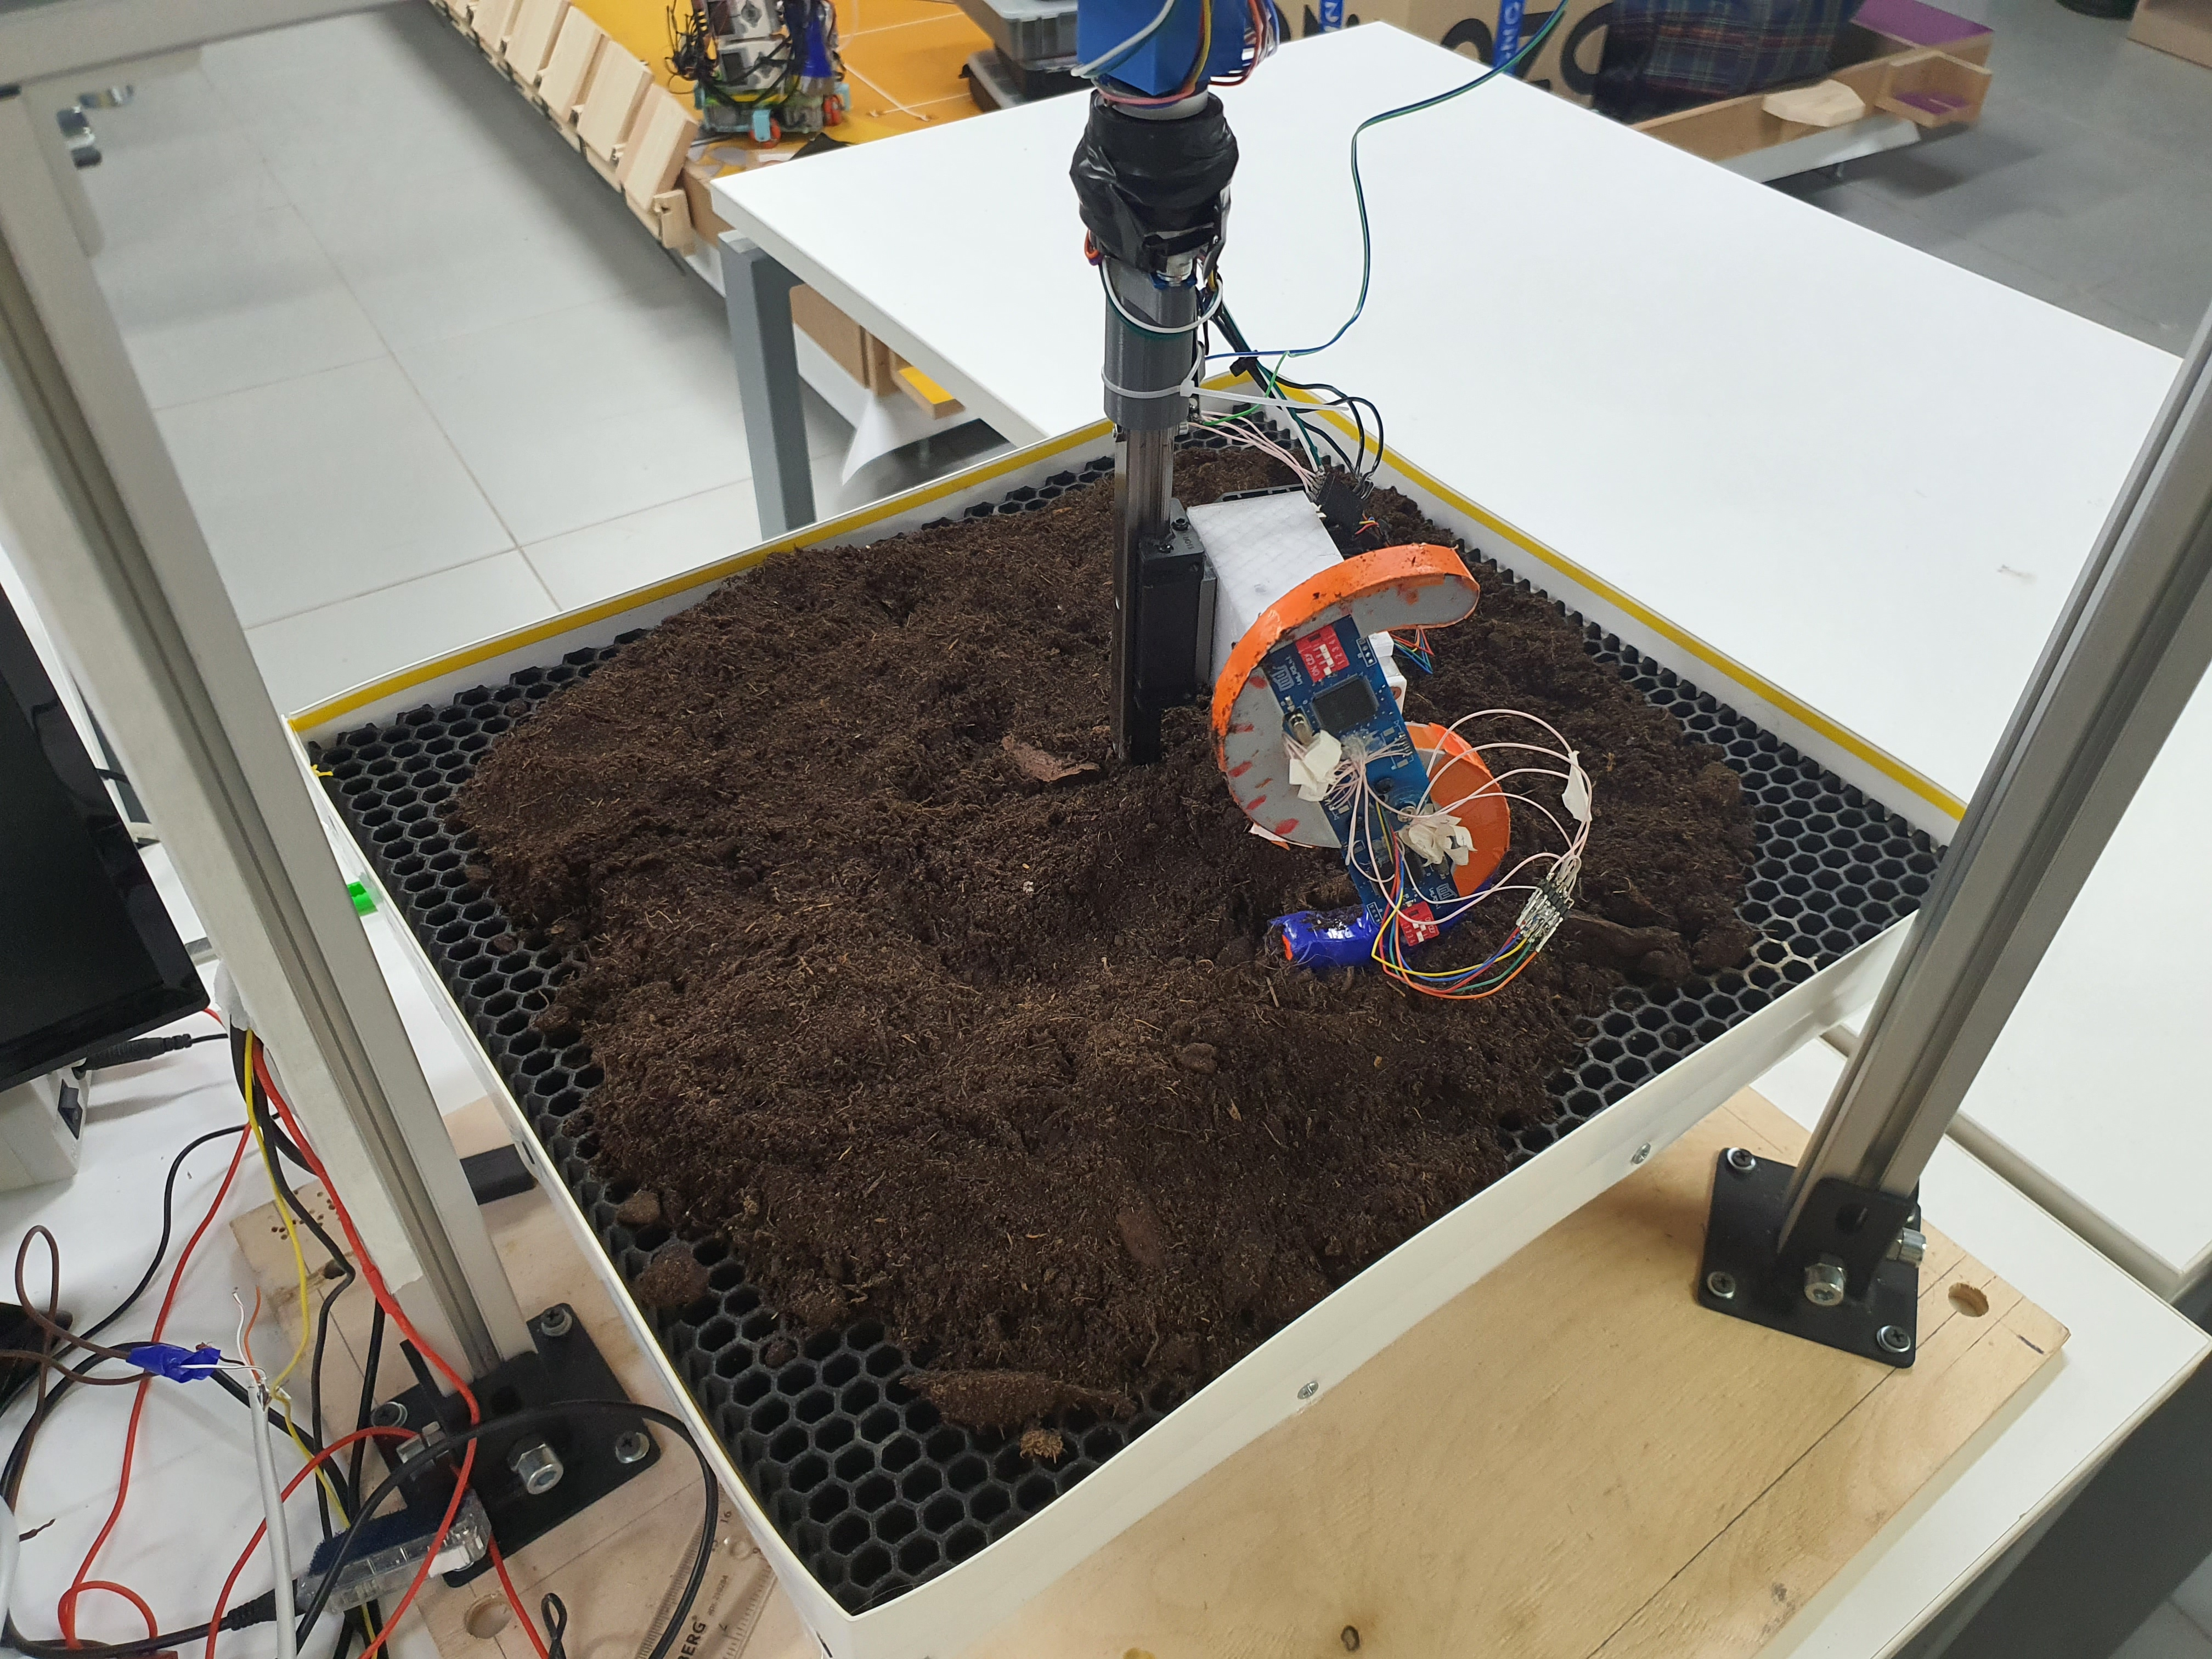
\includegraphics[height=9cm,width=1\textwidth,keepaspectratio]{s_shape_leg/mould.jpg}
        \caption{Земля}
        \label{fig:s_shape_leg/mould.jpg}
    \end{subfigure}
    \caption{Типы определяемых поверхностей}
\end{figure}

\begin{figure}[H]
    \centering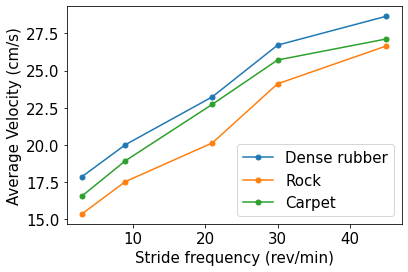
\includegraphics[height=8cm,width=1\textwidth,keepaspectratio]{s_shape_leg/avg_lin_vel_rev_min.png}
    \caption{Средняя линейная скорость робота}
    \label{fig:s_shape_leg/avg_lin_vel_rev_min.png}
\end{figure}

Были проведены замеры средней линейной скорости движения ноги на разных поверхностях при различных угловых скоростях \pic{fig:s_shape_leg/avg_lin_vel_rev_min.png}. Возможно заметить нелинейную зависимость, что так же может указывать косвенно на тип поверхности.

Ниже \pic{fig:data_from_legs} представлены необработанные данные с лапок робота. Сырые данные легко различить, но можно заметить, что абсолютные значения у разных сегментов различно. Поэтому при обучении необходимо их нормализовать.


\begin{figure}[H]
    \begin{subfigure}[t]{0.9\textwidth}
        \centering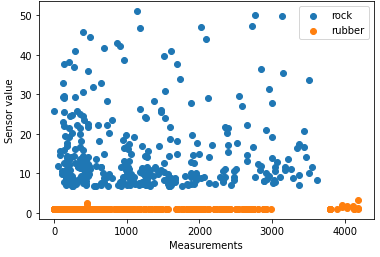
\includegraphics[height=6cm,width=1\textwidth,keepaspectratio]{s_shape_leg/segment8_compare_front.png}
        \caption{Передняя часть ноги, 8ой сегмент}
    \end{subfigure}

    \begin{subfigure}[t]{0.9\textwidth}
        \centering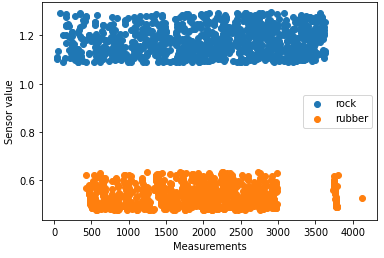
\includegraphics[height=6cm,width=1\textwidth,keepaspectratio]{s_shape_leg/segment6_compare_front.png}
        \caption{Передняя часть ноги, 6ой сегмент}
    \end{subfigure}
    \caption{Сравнение сырых данных после эксперимента с разных сегментов ноги}
    \label{fig:data_from_legs}
\end{figure}



\begin{figure}[H]
    \centering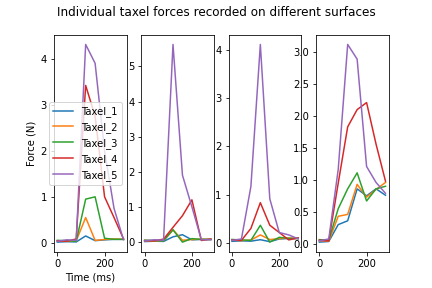
\includegraphics[height=8cm,width=1\textwidth,keepaspectratio]{s_shape_leg/TaxelIndForce.png}
    \caption{Запись активных такселей на разных поверхностях}
    \label{fig:s_shape_leg/TaxelIndForce_full.png}
\end{figure}

На рисунке выше \pic{fig:s_shape_leg/TaxelIndForce_full.png} представлены запись касания ногой на разных поверхностях. Можно заметить пиковую нагрузку на пятом такселе, на который приходится самый большой вес. На земле, по причине гранулированности поверхности, нагрузка более распределена. Это так же является хорошим критерием для определения типа поверхности

Применив предложенный алгоритм машинного обучения, данные с датчиков силы, а также массив угловых скорости были преобразованы с помощью Вейвлет-преобразования. Было проведено обучение, результатом которого получена таблица, представленная ниже \tab{tabular:prob_terrain_classification}.

\begin{table}[H]
    \caption{Вероятность определения типа поверхности}
    \label{tabular:prob_terrain_classification}
    \centering
\begin{tabular}{|c|c|c|c|c|} 
    \cline{3-5}
    \multicolumn{1}{l}{} & \multicolumn{1}{l|}{} & \multicolumn{3}{c|}{\textbf{Предсказанный класс}} \\ 
    \cline{3-5}
    \multicolumn{1}{l}{} &  & Резина & Камень & Земля \\ 
    \hline
    \multirow{3}{*}{{\textbf{Истинный класс}}} & Резина & {\cellcolor[rgb]{0.741,0.843,0.929}}84.0\% & 2.56\% & 13.44\% \\ 
    \hhline{|~----|}
     & Камень & 20.1\% & {\cellcolor[rgb]{0.741,0.843,0.929}}67.8\% & 12.1\% \\ 
    \hhline{|~----|}
     & Земля & 1.0\% & 18.9\% & {\cellcolor[rgb]{0.741,0.843,0.929}}80.1\% \\
    \hline
    \end{tabular}
\end{table}

Карта местности может быть построена с помощью 2D триангуляции Делоне (вогнутая оболочка). Входными данными для алгоритма является разреженное облако точек касаний робота поверхности, собранные с помощью преобразователя силы на основе Velostat.

Точность, полученная в симуляторе равна примерно 5 см, а во время натурного эксперимента -- 8 см, что является адекватным результатом для поставленной задачи.

С помощью разработанного преобразователя силы возможно различать 3 типа поверхности: резину, землю и каменистую гряду.